\section{Path Planning}

\begin{frame}{Informative Path Planning}{Information measurement}
\begin{itemize}
\item minimize the uncertainty of the observed environment
\end{itemize}
\begin{figure}
	\centering
	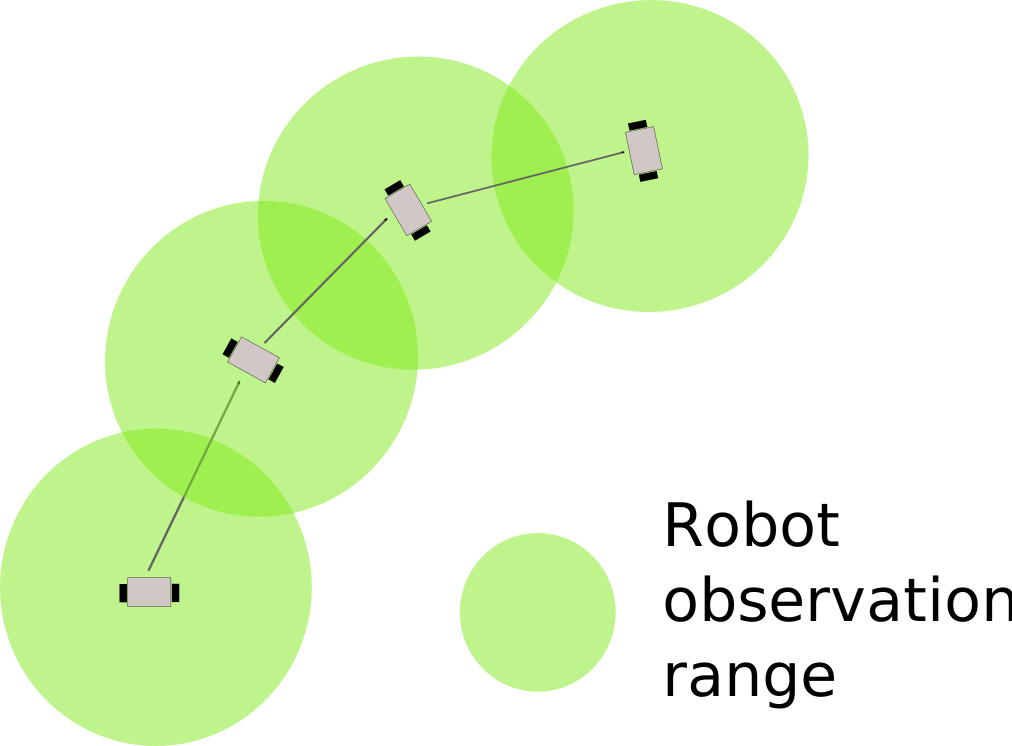
\includegraphics[width = .6\textwidth]{./figure/robotObservation}
\end{figure}
\end{frame}

\begin{frame}{Cordon and search}{Application}
\begin{columns}
	\column{0.5\textwidth}
	\begin{minipage}{\textwidth}
		\begin{figure}
			\centering
			\includegraphics[width = 0.9\textwidth]{./figure/cordon_and_search.jpg}
		\end{figure}
	\end{minipage}
	
	\column{0.5\textwidth}
	\begin{minipage}{\textwidth}
		\begin{figure}
			\centering
			\includegraphics[width = 0.9\textwidth]{./figure/soldier_and_robot.jpg}
		\end{figure}
	\end{minipage}	
\end{columns}
\end{frame}

\begin{frame}{Map discretization}{Application}
	\begin{columns}
		\column{0.5\textwidth}
		\begin{minipage}{\textwidth}
			\begin{figure}
				\centering
				\includegraphics[width = 0.9\textwidth]{./figure/map_tld_europe.jpg}
			\end{figure}
		\end{minipage}
		
		\column{0.5\textwidth}
		\begin{minipage}{\textwidth}
			\begin{figure}
				\centering
				\includegraphics[width = 0.9\textwidth]{./figure/hexagonal_europe_map.png}
			\end{figure}
		\end{minipage}	
	\end{columns}
\end{frame}

\begin{frame}{Submodular orienteering}{Informative path}
	
	\begin{block}{Conditional mutual information}
		$ I(\mathbf{S}; \mathbf{O}^{X} \mid \mathbf{O}^{Y^{h}}) = H(\mathbf{S} \mid \mathbf{O}^{Y^{h}}) - H(\mathbf{S} \mid \mathbf{O}^{X},\mathbf{O}^{Y^{h}}) $
	\end{block} 
	
	\bigskip
	
	\begin{itemize}
		\item Entropy reduction
		\item Submodularity
		\item Chain rule \\
		$ I(\mathbf{S}; \mathbf{O}^{X} \mid \mathbf{O}^{Y^{h}}) = \sum_{t=1}^{T} I(O^{X}_{t} ; \mathbf{S} \mid O^{X}_{1} , \cdots , O^{X}_{t-1}, \mathbf{O}^{Y^{h}}) $
	\end{itemize}
	
\end{frame}

%\subsection{Human constraint}

\begin{frame}{Team role}{Human constraint}
	
	\begin{figure}
		\centering
		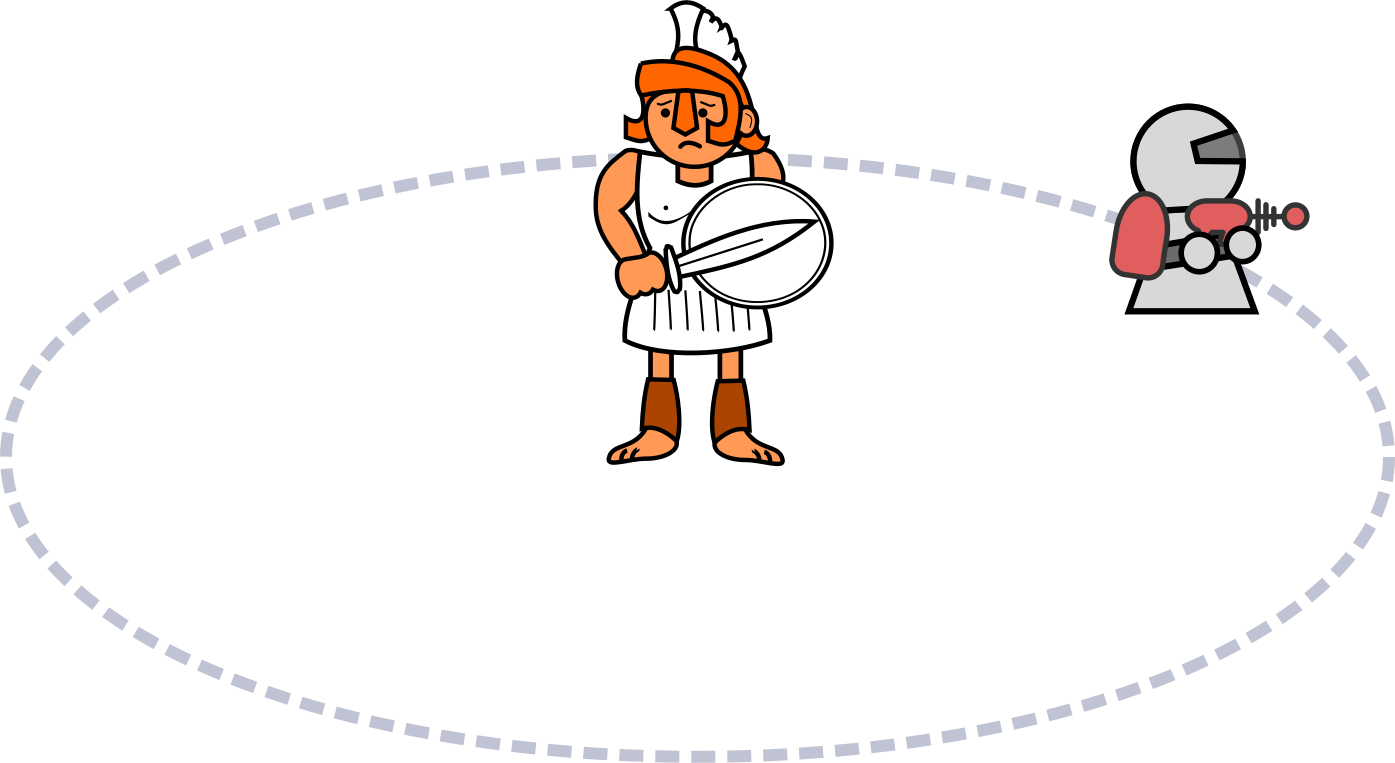
\includegraphics[width = 0.7\textwidth]{./figure/human_robot_interaction}
	\end{figure}
	
	\begin{itemize}
		\item cooperative observation
		\item assistance and protection
	\end{itemize}
	
\end{frame}

\begin{frame}{Neighboring function}{Human constraint}
	\begin{columns}
		\column{.6\linewidth}
		\begin{minipage}[c]{\linewidth}
			\begin{figure}
				\centering
				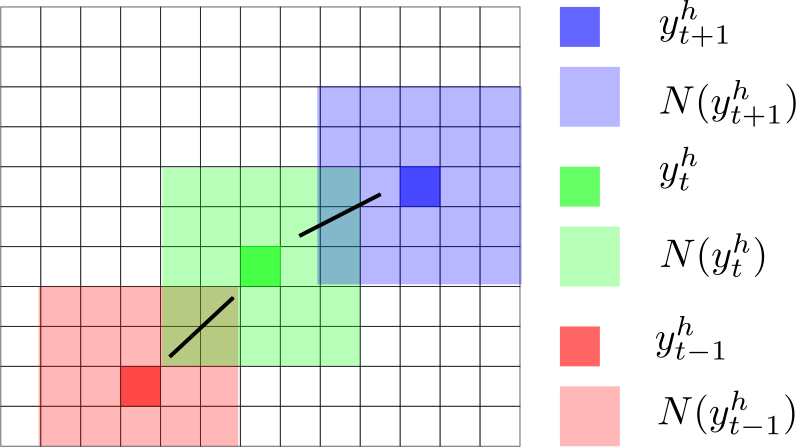
\includegraphics[width = \textwidth]{./figure/humanConstraint}
				%\caption{An example of human constraint.}
			\end{figure}
		\end{minipage}
		
		\column{.4\linewidth}
		\begin{minipage}[c]{\linewidth}
			\begin{itemize}
				\item { human path $ \{ y^{h}_{1} \cdots y^{h}_{T} \} $ }
				\item { neighboring function $ N( y^{h}_{t} ) $ }
			\end{itemize}
		\end{minipage}
	\end{columns}
	
\end{frame}

\begin{frame}{Related work}{ Using a greedy heuristic}
\begin{block}{A}
	content...
\end{block}
\begin{block}{B}
\end{block}
\end{frame}

\begin{frame}{Related work}{Using a multi-resolution dynamic programming}
	|
\end{frame}




